\section{Surface Quasi-Geostrophic Turbulence}
\label{sec:sqg}

Our goal in this study is to emulate turbulent motions relevant to realistic
geophysical fluid dynamics, while avoiding the complications
associated with the data assimilation system choices required for reanalyses
and the intricate multivariate interactions inside atmosphere or ocean GCMs.
Therefore, we aim to emulate a numerical model for
SQG turbulence as outlined by \citet{tulloch_note_2009}.
The model is formulated to represent the nonlinear Eady problem
\citep{eady_long_1949}, following \citet{blumen_uniform_1978-1}.
The model simulates turbulence
on an $f$ plane with uniform stratification and shear, bounded by rigid
surfaces $H=10$~km apart.
The motion is determined entirely by temperature advection on the boundaries
$z=\{0\text{~km},10\text{~km}\}$ as follows,
\begin{equation*}
    \dfrac{\partial \hat{\theta}}{\partial t} +
    \hat{J}(\hat{\psi}, \hat{\theta}) + ik\left(U \hat{\theta} +
        \hat{\psi}\dfrac{\partial \Theta}{\partial y}\right)
    = 0 \qquad z = 0, 10\,\text{km} \, ,
\end{equation*}
where $z=0$~km is the surface layer of the atmosphere, and $z=10$~km is
approximately at the top of the troposphere.
Here, hatted variables denote spectral components, $\hat{J}$ is the Jacobian in
spectral space, and the temperature streamfunction is
\begin{equation*}
    \hat{\psi}(z,t) = \dfrac{H}{\mu\sinh\mu}
    \left[ \cosh\left(\mu\dfrac{z}{H}\right) \hat{\theta}(H,t)
        - \cosh\left(\mu\dfrac{z-H}{H}\right) \hat{\theta}(0,t)
    \right]\, ,
\end{equation*}
with $\mu = |\mathbf{K}| NH/f$ as the nondimensional wavenumber.
We note that this model produces an approximate spectrum of
$|\mathbf{K}|^{-5/3}$ without any break,
as is expected in Eady turbulence (\cref{fig:sqg-reference}).
For more details on this model, see \citep{tulloch_note_2009}.


\begin{figure}
    \centering
    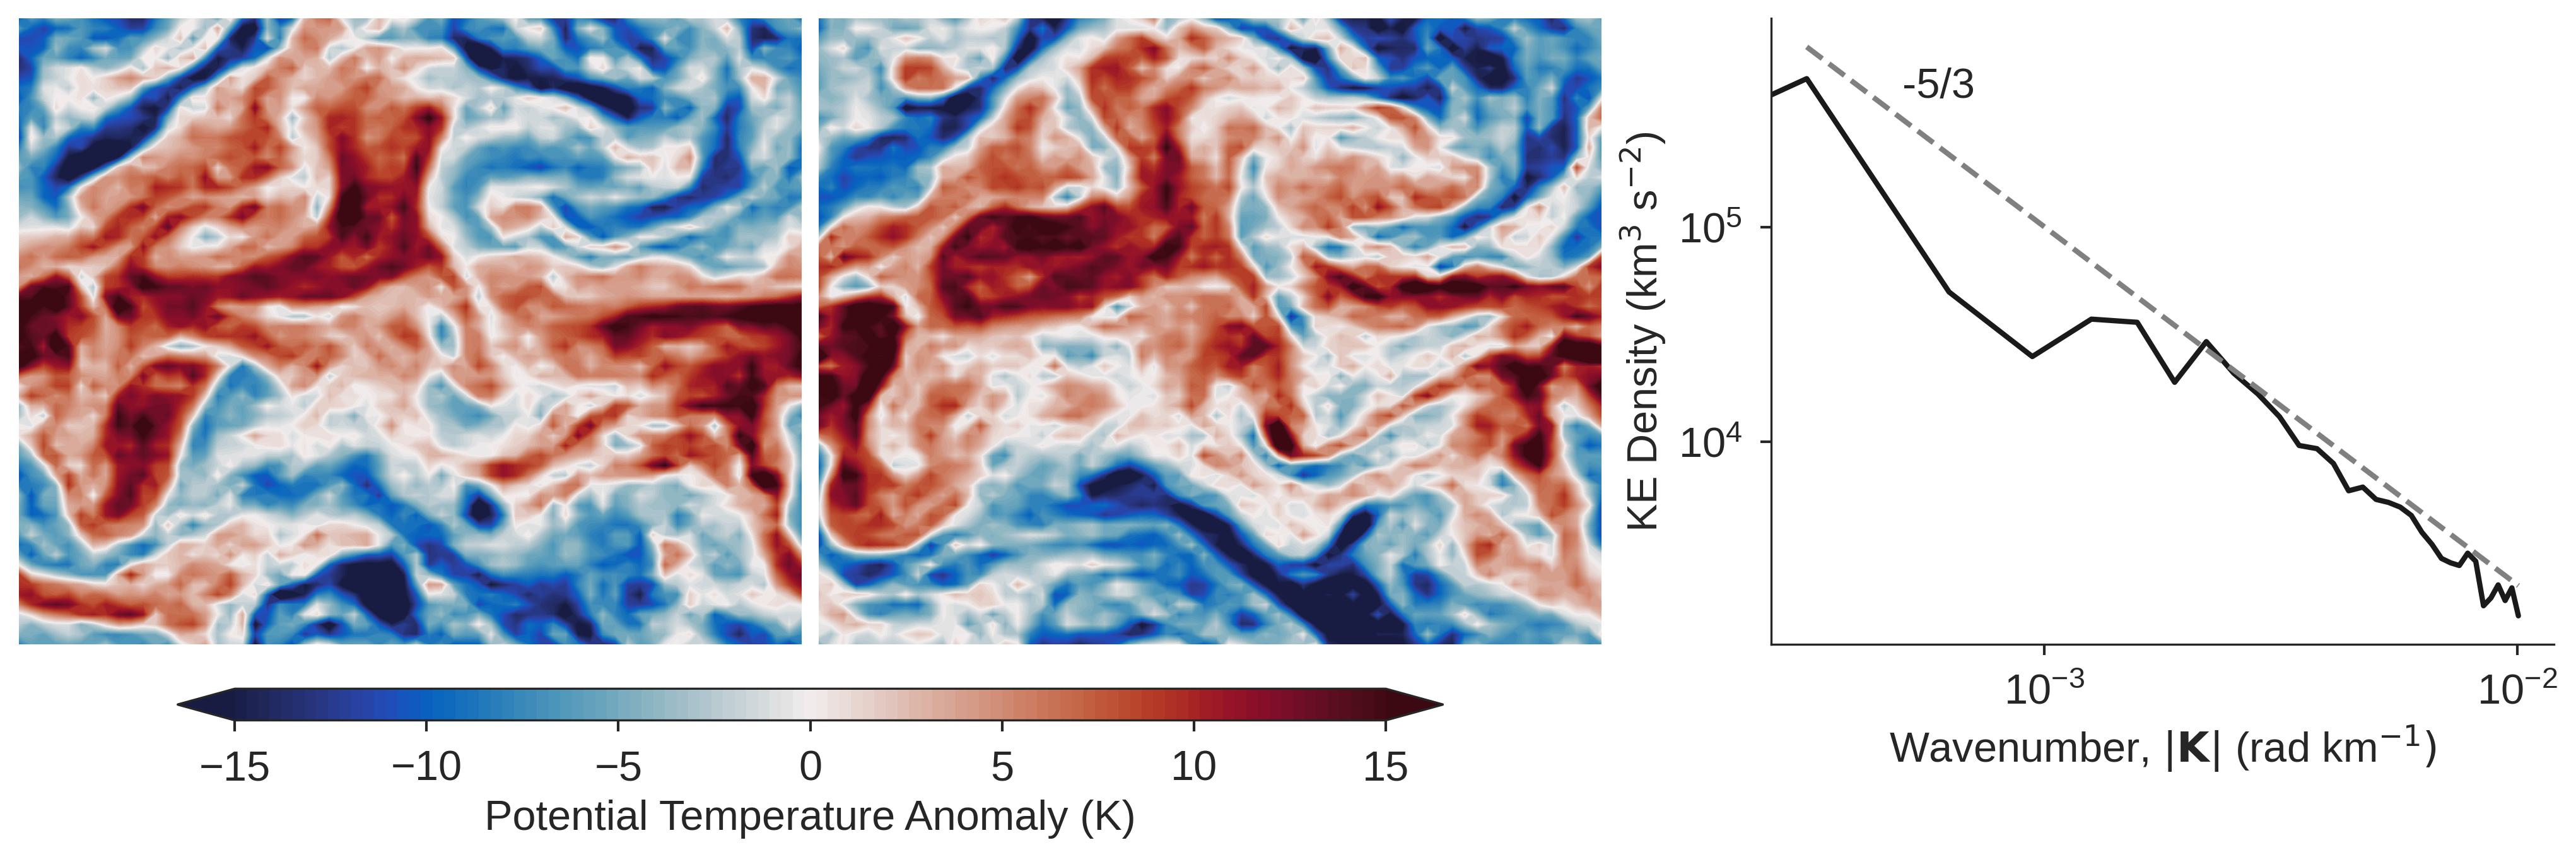
\includegraphics[width=\textwidth]{../figures/sqg_reference_plot.jpg}
    \caption{A reference snapshot from the SQG dataset. The left and middle panels
        show snapshots of potential temperature anomaly at the surface and
        top-of-troposphere layers, i.e. at a height of 10~km, respectively.
        The right panel shows the kinetic energy density spectrum associated
        with this snapshot (black line), compared to
        $|\mathbf{K}|^{-5/3}$ (dashed line).
    }
    \label{fig:sqg-reference}
\end{figure}

The model is discretized in space with $N_x = N_y = 64$, and uses a timestep of
$\Delta t=5$~minutes.
To generate datsets for the neural networks, we initialize the model with Gaussian i.i.d.
noise and spinup for 360~days, which we define as one model year.
The spinup period is discarded, and we then generate a 25~year dataset that we partition
into training (first 15~years), validation (following 5~years), and testing
(final 5~years).
For validation and testing, we randomly select 12~hour time windows from each
respective dataset.
